% !TEX program = xelatex
% ---------------------IMPORTS---------------------
\documentclass[en, screen, 12pt]{article}
\usepackage{graphicx} % Required for inserting images
\usepackage{hyperref}
\usepackage{titlesec}
\usepackage{svg}
\usepackage[utf8]{inputenc}
\usepackage{datetime} % Date time package
\usepackage{fancyhdr} % For custom headers and footers
\usepackage[a4paper, margin=1in, headsep=0.5in]{geometry} % Set all margins to 1 inch
\usepackage{lastpage} % For getting the total number of pages
\usepackage{lipsum}
\usepackage{enumitem}
\usepackage{acronym}
\usepackage{float}
\usepackage{caption} 

% Set Garamond as main font
\usepackage{fontspec}
\setmainfont{EB Garamond}

\usepackage[
    backend=biber,
    style=ieee,      % or "numeric", "authorylatear", etc. if you want like APA
    sorting=ynt
]{biblatex}

\addbibresource{References/references.bib} % Bib file with your references

% Set line spacing to 1.5 (common in research papers)
\linespread{1.5}

% Global settings for all lists
% \setlist{itemsep=0pt, topsep=0pt, parsep=0pt, partopsep=0pt}
\setlist{itemsep=0pt}

% \usepackage{geometry} % Adjust page margins etc.

% ---------------------UNCOMMENT FOR DARK MODE---------------------
% \usepackage{xcolor}
% \pagecolor[rgb]{0,0,0} %black
% % \color[rgb]{255,255,255} %text white
% \color[rgb]{0.827,0.827,0.827} %text color grey

% ---------------------DOCUMENT VARIABLES ---------------------
\newcommand{\doctitle}{Electric Propulsion Thruster for Nanosatellites} % EDIT THIS TO CHANGE TITLE !!!!!!
\newcommand{\VersionNumber}{Version : 1.0.0} % EDIT THIS TO CHANGE VERSION !!!!!!


% ---------------------STYLING AND DOC SETUP ---------------------
% COLORS
\definecolor{red}{RGB}{255,0,0}
\definecolor{grey}{RGB}{211,211,211}

% HYPERLINKS
\hypersetup{
    colorlinks=true,
    urlcolor=black,
    linkcolor=black,
    citecolor=black
}

% DATEFORMAT
\newdateformat{mydate}{\THEDAY\ \monthname[\THEMONTH], \THEYEAR}

% ---------------------HEADER SETUP---------------------
\pagestyle{fancy}
\fancyhead[L]{
\includegraphics[height=15pt]{images/ASTROPULSE.png}} % Logo in top left
\fancyhead[R]{\doctitle} % Page number in top right
\fancyfoot[C]{Page \thepage\ of \pageref{LastPage}}
\renewcommand{\headrulewidth}{1.0pt}

\renewcommand{\headrule}{\hbox to\headwidth{\color{black}\leaders\hrule height \headrulewidth\hfill}}

% ---------------------TITLE SETUP---------------------
% Redefine \maketitle to include the image
\makeatletter
\renewcommand{\maketitle}{
  \begin{titlepage}
    \null\vfill
    \centering
    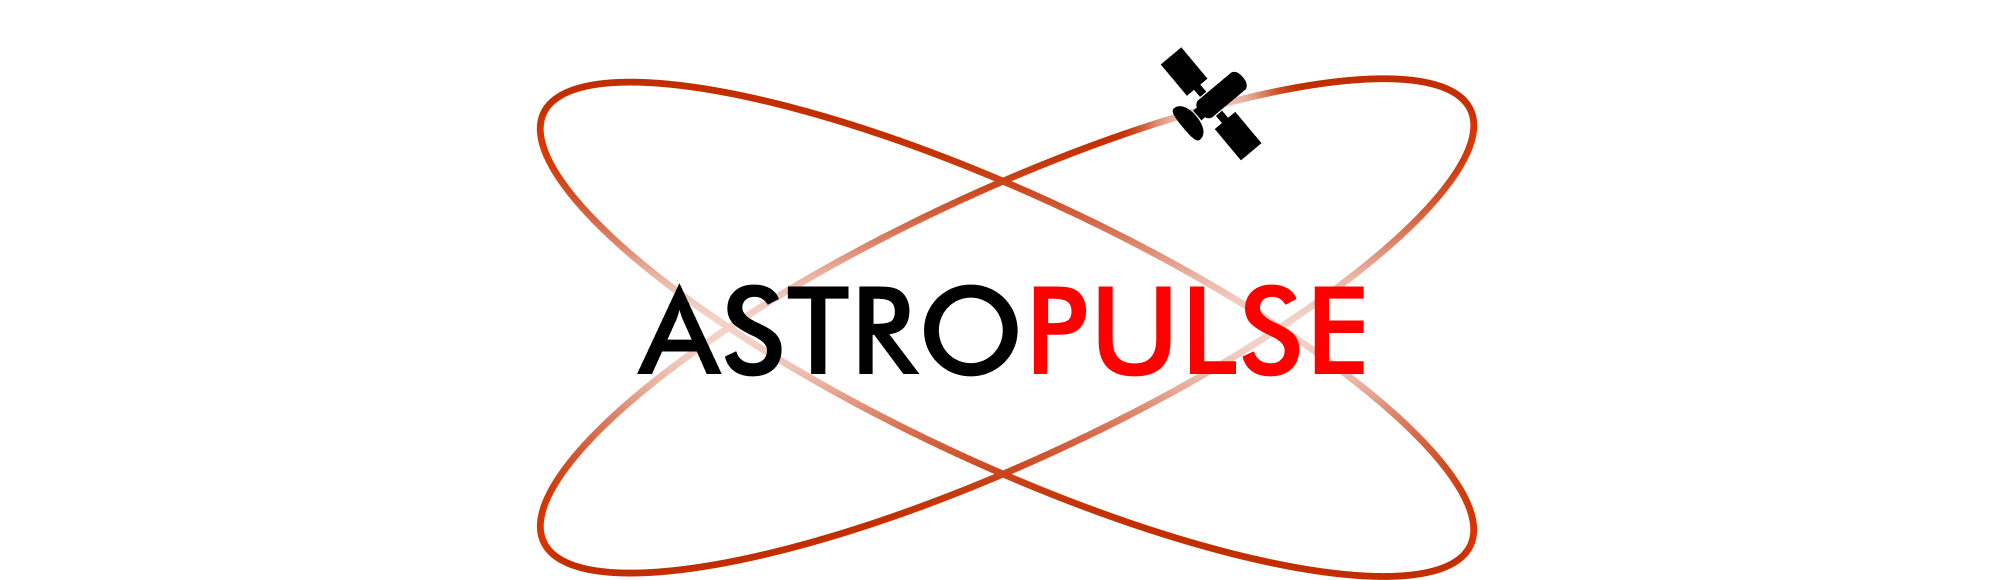
\includegraphics[width=1.0\textwidth]{images/ASTROPULSE LOGO.png}
    \par\vspace{2em}
    {\Huge\bfseries\@title\par}
    \vspace{1.5em}
    {\Large\@author}
    \par\vspace{2em}
    {\Large\@date}
    \par\vspace{2em}
    {\Large\VersionNumber}
    \vfill

    % \textbf{Revision Table}
    % ------REVISION TABLE------
    %\begin{table}[htbp]
    %     \centering
    %     \begin{tabular}{|c|c|c|c|c|}

    %         \hline
    %         \textbf{Version} & \textbf{Author(s)} & \textbf{Changes} & \textbf{Approved By} & \textbf{Date} \\
    %         \hline

    %          &  &  &  &  \\
    %         \hline

    %          &  &  &  &  \\
    %         \hline
    %     \end{tabular}

    %     \label{tab:revision table}
    % \end{table}
    
    \null
  \end{titlepage}
}
\makeatother

% ---------------------TITLE CONTENT---------------------
\title{Group 17 \\ \doctitle}
% \author{Authors : Author Names}
\author{
Shivam S. Desai, 
Andrew C. Gonsalves, 
Gurnoor Gill, \\
Zachariah T. Blair,
Zachary A. Scott,
Gavin Angstad
}

\date{Date : \mydate\today}

% ---------------------END OF SETUP---------------------

% \includeonly{
%   content/Project Overview/Introduction.tex,
%   content/Project Overview/Deliverables and Objectives.tex
% }

% ---------------------START OF DOCUMENT---------------------
\begin{document}

% ---------------------TITLE PAGE---------------------
\maketitle

% ---------------------ABSTRACT---------------------
% UNCOMMENT IF YOU WANT AN ABSTRACT !!!!
% \include{content/abstract}

% ---------------------TABLE OF CONTENTS---------------------
\newpage
\tableofcontents
\newpage

% ---------------------ACKNOWLEDGEMENTS---------------------
\section*{Acknowledgments}

Shoutouts to people who helped us

% ---------------------ABBREVIATIONS---------------------
\newpage
\section*{List of Abbreviations}
\begin{acronym}
    \acro{GEO}{Geostationary Orbit}
    \acro{MEO}{Medium Earth Orbit}
    \acro{LEO}{Low Earth Orbit}
    \acro{EP}{Electric Propulsion}
    \acro{CSA}{Canadian Space Agency}
\end{acronym}

% ---------------------NOMANCLATURE---------------------
\newpage
\section*{NOMANCLATURE}
\begin{acronym}
    \acro{$A_e$}{Thruster exit area [m$^{2}$]}
\end{acronym}

% ---------------------------------------------------------
% \setcounter{page}{1} % Start page numbering

% ---------------------CONTENT---------------------

% PROJECT OVERVIEW
\section{Project Overview}

\subsection{Introduction}

\subsubsection{Background}

The first satellite, Sputnik 1, was launched by the Soviet Union on October 4, 1957. This event marked the start of the space race, leading to new technological, scientific, and political developments \cite{nasa-sputnik}. Since then, 23030 satellites have been launched \cite{esa-debris}. Satellites orbiting Earth can be split into 3 catagories:

\begin{itemize}
    \item \ac{LEO} : 160 km - 2,000 km

    \item \ac{MEO} : 2,000 km - 35,786 km

    \item \ac{GEO} : 35,786 km
\end{itemize}

For decades interest lied in \ac{GEO} satellites, with Syncom becoming the first \ac{GEO} satellite in 1963~\cite{nasa-syncom}. Being in geosynchronous orbit meant that satellites could stay at a specific position above Earth, allowing for constant communication with a specific area on Earth. This made these satellites ideal for communication and weather monitoring. However, \ac{GEO} satellites have high latency due to their distance from Earth, making them less suitable for real-time applications.

Since then the most significant change in satellite technology has been the development of \ac{LEO} satellites. Although they were first developed in the 1990s, these satellites have only really become widely used in the last decade. Companies like OneWeb and Starlink have launched constellations of \ac{LEO} satellites to provide low-latency internet access across the globe~\cite{reliasat-evolution}. These developments denoted a transition in the commercial communication satellite business from small numbers of large geostationary satellites towards constellations of hundreds of smaller lower satellites in low earth orbit.

Fueled by this new idea, the global space industry accelerates as the number of satellites launched annually continues to rise. Both governments and private entities are allocating significant resources to satellite research and development for applications such as communication, navigation, Earth observation, atmospheric characterization, and military purposes.

\subsubsection{Project Motivation}

With the increasing complexity of mission requirements, the need for more advanced satellite technologies has increased. Specifically, the need for efficient and reliable propulsion systems has become crucial for satellite operations. Satellites require propulsion for various reasons, including orbit insertion, station-keeping, attitude control, deorbiting at the end of their operational life, and formation flying. Additionally, as spent rockets, satellites and other space trash accumulate in orbit, the likelihood of collisions with debris has increased. Unfortunately, collisions create more debris creating a runaway chain reaction of collisions and more debris known as the Kessler Syndrome~\cite{nasa-kessler}.

There are two main types of propulsion systems used in satellites: chemical propulsion and \ac{EP}. Satellites have traditionally used chemical propulsion systems, although there is now a huge shift towards \ac{EP} systems with Space X's Starlink constellation being the largest adopter of EP technology.

Chemical propulsion uses a fuel and an oxidizer, converting energy stored in the chemical bonds of the propellants, to produce a short, powerful thrust, or what we see as fire. It’s loud and exciting, but not all that efficient. Chemical propulsion is said to be "energy limited" because the chemical reactants have a fixed amount of energy per unit mass, which limits the achievable exhaust velocity or \ac{$I_{sp}$}.

Electric propulsion systems use energy collected by either solar arrays or a nuclear reactor to generate thrust by using electric, and possibly magnetic, processes to ionize and accelerate a propellant. It is a technology aimed at achieving thrust with high-exhaust velocities, which results in a reduction in the amount of onboard propellant required for a given space mission or space-propulsion application compared to other conventional propulsion methods. Reduced propellant mass can significantly decrease the launch mass of a spacecraft or satellite, leading to lower costs from the use of smaller launch vehicles to deliver a desired mass into orbit or to a deep space target. \cite{fundamentals-of-electric-propulsion}
It can reduce the amount of fuel, or propellant, needed by up to 90\% compared to chemical propulsion systems, saving millions in launch costs while providing greater mission flexibility. \cite{nasa-electrifying-propulsion}

\begin{figure}[H]
    \centering
    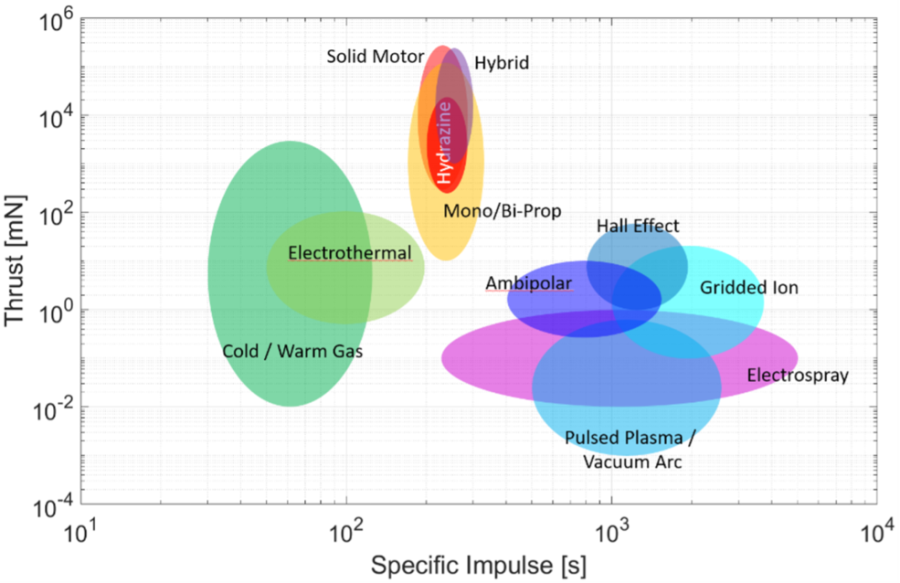
\includegraphics[width=0.9\textwidth]{images/Concepts/thrust vs specific impulse for electric systems.png}
    \captionsetup{justification=centering}
    \caption{Typical small spacecraft in-space propulsion (thrust vs specific impulse) \\ Chemical Thrusters shown in shades of red and Electric Thrusters shown in shades of blue\cite{nasa-inspace-propulsion}.}
    \label{fig:thrust_vs_specific_impulse_propulsion_systems}
\end{figure}

\subsubsection{Relevance}

As the technology matures and becomes more widely adopted, we can see an increasing interest in the space and satellite industry by the goverment of Canada. The \ac{CSA} has been actively encouraging development in the industry through initiatives such as the "Call for Ideas - Science and technology small payloads for space missions"~\cite{csa-call-for-ideas}. The \ac{CSA} also initated a "Consultation on Changes to Licensing Requirements and Conditions of Licence on Space Debris Mitigation" \cite{csa-space-debris-mitigation}, which aims to address the growing concern of space debris. It proposes mandating active propulsion systems, with redundancy, for all Non-Geostationary Satellite Orbit (NGSO) satellites operating at or above 400 kilometers. This can severley increase the system and integration complexity for small satellites. Hence, now more than ever, there is a need to develop modern, efficient, and reliable propulsion systems for satellites. This shows that the goverment of Canada is aware of the increasing importance of the space industry and is taking steps to ensure its growth and sustainability.


\section{Capstone Outline}
To tackle these issues this capstone project aims to explore the design, simulation, and prototyping of an electric propulsion system suitable for nanosatellites (1–10 kg). First a suitable method of electric propulsion will be selected based on mission requirements and compatibility with nanosatellite applications. The team will then design an electric propulsion module consisting of the key subsystems: a \ac{PPU}, a propellant storage and feed system, an ionization system.

The proposed design will evaluated using simulation softwares to assess performance metrics such as thrust, electrical performance, and orbital maneuvering potential. Finally, the team will develop a ground-based test stand prototype. While thruster testing may not be possible, this will lay the framework to measure and analyze critical parameters such as thrust, specific impulse, efficiency, and overall system stability under representative operating conditions.

\section{Capstone Requirements}
The primary requirements for the electric propulsion system are as follows:
\begin{itemize}
    \item The propulsion system must be compatible with nanosatellite platforms in the 1–10 kg range
    \item The propulsion module should fit within a volume of 3U (30 cm x 10 cm x 10 cm) or smaller
    \item The system should be capable of producing a thrust level sufficient for orbit keeping of a nanosatellite at 200km altitude
    \item The total power consumption of the propulsion system should not exceed 500W
    \item The system should provide a $I_{sp}$ greater than 500 seconds
    \item The propulsion system and \ac{PPU} should not exceed a total mass of 3kg
    \item The propulsion system should utilize a propellant that is safe and easy to handle
    \item The design should include considerations for thermal management to ensure stable operation in space environments
\end{itemize}

\section{Capstone Deliverables}

The expected deliverables are as follows:

\begin{itemize}
    \item A prototype electric propulsion module suitable for nanosatellites in the 1–10 kg range
    \item A design and prototype of a thrust test stand capable of accurately measuring low thrust levels
    \item CAD models, technical drawings, and electronic schematics associated with the system
    \item Simulation results validating key aspects of the propulsion system, including thrust and electrical performance
\end{itemize}

These outcomes will demonstrate the feasibility of implementing electric propulsion on nanosatellite platforms and provide a foundation for further development and testing	


% CONCEPTUAL DESIGN
\section{Conceptual Design}

% INSTRUCTIONS FOR NOW
In this section make sure to:
\begin{itemize}

    \item Explain Past Methods (eg. from reseach papers)

    \item Your concept

    \item Why your concept
\end{itemize}
% -----------------------------------------

\subsection{System Overview}


% Currently this contains examples
% Replace with real content
Einstein’s work on relativity changed physics forever \cite{einstein1905}.
Knuth’s book is a classic in computer science \cite{knuth1984}.
% -----------------------------------------

% Thruster Design
\section{Hall Thruster Types}
\subsection{Annular Hall Thrusters}
\ac{AHT}s are the most common type of \ac{HET} in use today. They feature an axisymmetrical annular discharge channel where the propellant is ionized and accelerated. The magnetic field is generated by coaxial coil windings wrapped in and around the discharge channel or by permanent magnets. It consists on a high voltage metallic anode located upstream in the channel, and a cathode that is often located outside the channel.

In-space thruster tests with this geometry have demonstrated thrusts up to 280mN. They have exhibited power levels of up to 4.5kW, and specific impulses up to 2000s. \cite{bpt-4000} \cite{spt-140} \\

\begin{figure}[H]
    \centering
    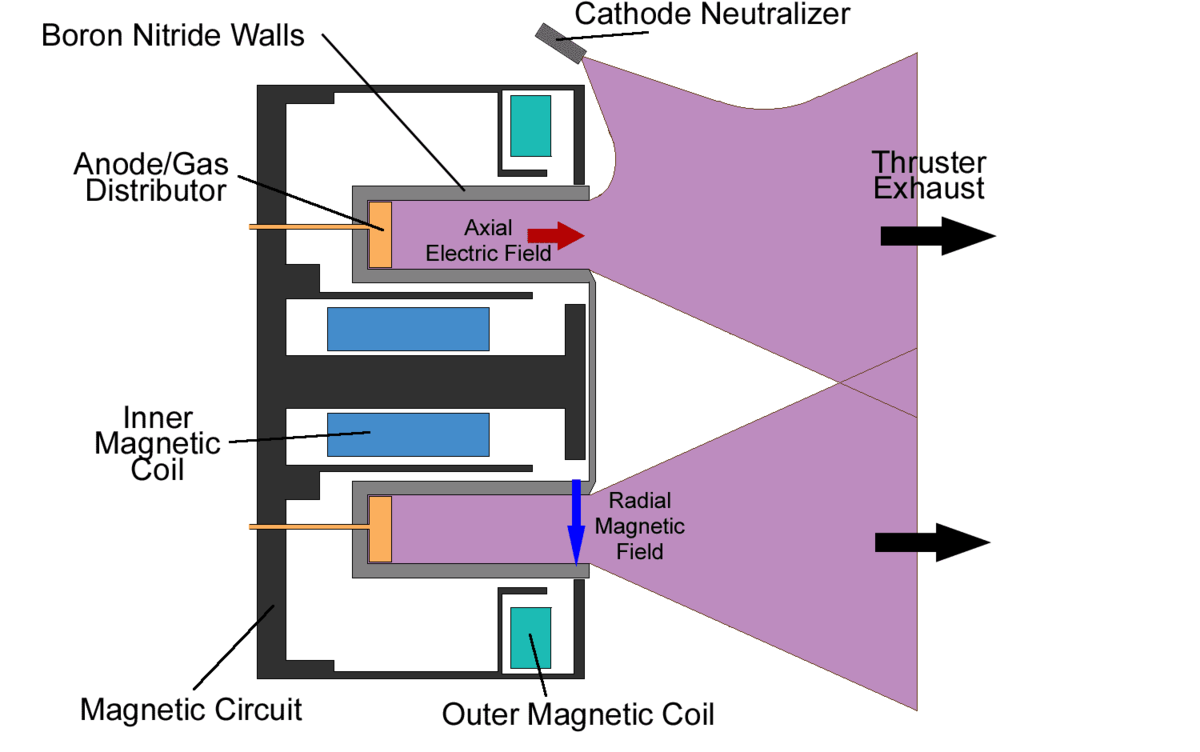
\includegraphics[width=0.7\textwidth]{images/Concepts/Annular HET.png}
    \captionsetup{justification=centering}
    \caption{Annular \ac{HET}}
    \label{fig:annular_HET}
\end{figure}


\subsection{Cylindrical Hall Thrusters}

One of the largest drawbacks when downscaling \ac{AHT}s is the increase in surface area to volume ratio, which leads to higher wall losses and lower efficiency. The plasma tends to interact with the thruster channel walls, which results in heating and erosion of the thruster parts \cite{cht-plasma-wall-interactions}. To combat this, \ac{CHT}s, proposed at the Princeton Plasma Physics Laboratory were developed. As seen in figure \ref{fig:cylindrical_HET}, the ratio of the channel surface area to volume is reduced, limiting electron transport and ion losses \cite{pppl-cht}. These thrusters have also seen unusually high propellant ionization efficiencies, hence being able to operate at much lower discharge voltages and propellant flow rates \cite{cht-vs-aht}. These thrusters are often developed at much smaller scales, generally thrusters with a diameter of less than 50mm. While they have produced statistics comparable to annular thrusters in the lab environment, they are yet to be flown in space.

\begin{figure}[H]
    \centering
    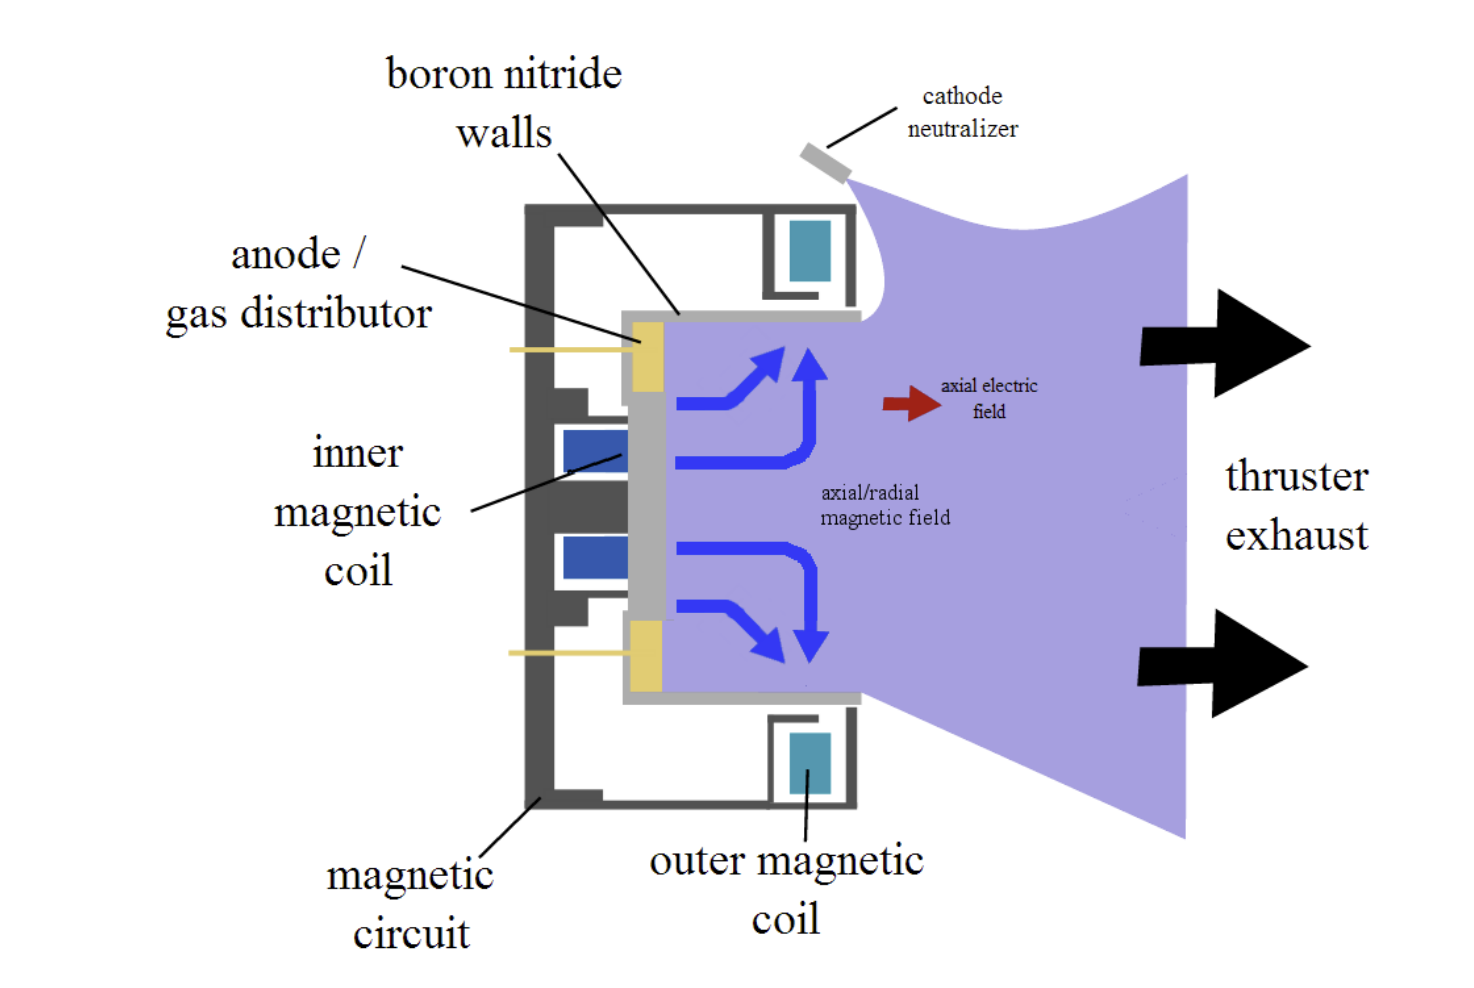
\includegraphics[width=0.7\textwidth]{images/Concepts/CHT.png}
    \captionsetup{justification=centering}
    \caption{Cylindrical \ac{HET} \cite{pigeon2017development}}
    \label{fig:cylindrical_HET}
\end{figure}
\subsubsection{Propellant Selection}
\section{Propellant Feed System and Anode}

storage tank
feed plumbing
injector

talk about anode


\include{content/Conceptual Design/Thruster Design/Channel Ablative.tex}
\section{Magnetic Field Design}
\subsubsection{Cathode}

% Avionics
\section{Avionics}

To control and operate the thruster we require an avionics subsystem that can provide power, control signals, and data acquisition. For this several \ac{PCB}s may need to be designed such as the \ac{PPU}, and a seperate low power control board. Accompanying, this electrical system a real time software control system will be needed to operate the thruster, and monitor its performance. 


% Explain high level what is needed in the avionic substem

% Include high level / block diagrams

% Explain that real time software control will be needed
\subsubsection{Electrical System}

block diagrams
reference to existing designs
explanation of the goal of the system
how it will be run from soalr panels
etc

\subsection{Software}

reference to existing use of real time system in rockets
Exaplin the RTOS
and using MCU peripherals like PWM
How this choice of software architecture will help achieve the final goals
Explain that low power feature will be used to minimize power consumption in space

% Testing
\section{Testing}

\subsection{Testing in Vaccum}

Talk about chamber and testing considerations

\subsection{Test Stand}

explain existing methods

why you chose yours

touch on initial concept

change dues to chamber sizes

final concept

data acquisiton needed





\section{Final Concept}

The final basic geometry of our final concept is shown in figure \ref{fig:final_concept}. It is important to note that the render does not include all components such as the propellant feed system and propellant diffuser, and that the design may very well change as we move through the design process. However, it does the job of conveying some of the design goals and choices that have been made. The final concept will consist of the following features:

\begin{enumerate}
    \item Magnetic Field System - will consist of a ferromagnetic core with permanent magnets to create the required magnetic field topology. This will reduce power consumption and
    avionics system complexity
    \item Cathode - will be centrally mounted on the thruster axis allowing for a more compact design
    \item Ring anode - simple and well understood design
    \item Propellant feed system - will consist of a pressure vessel, custom propellant diffuser, and supporting hardware. May become to primary conductor to the anode.
\end{enumerate}

\begin{figure}[H]
    \centering
    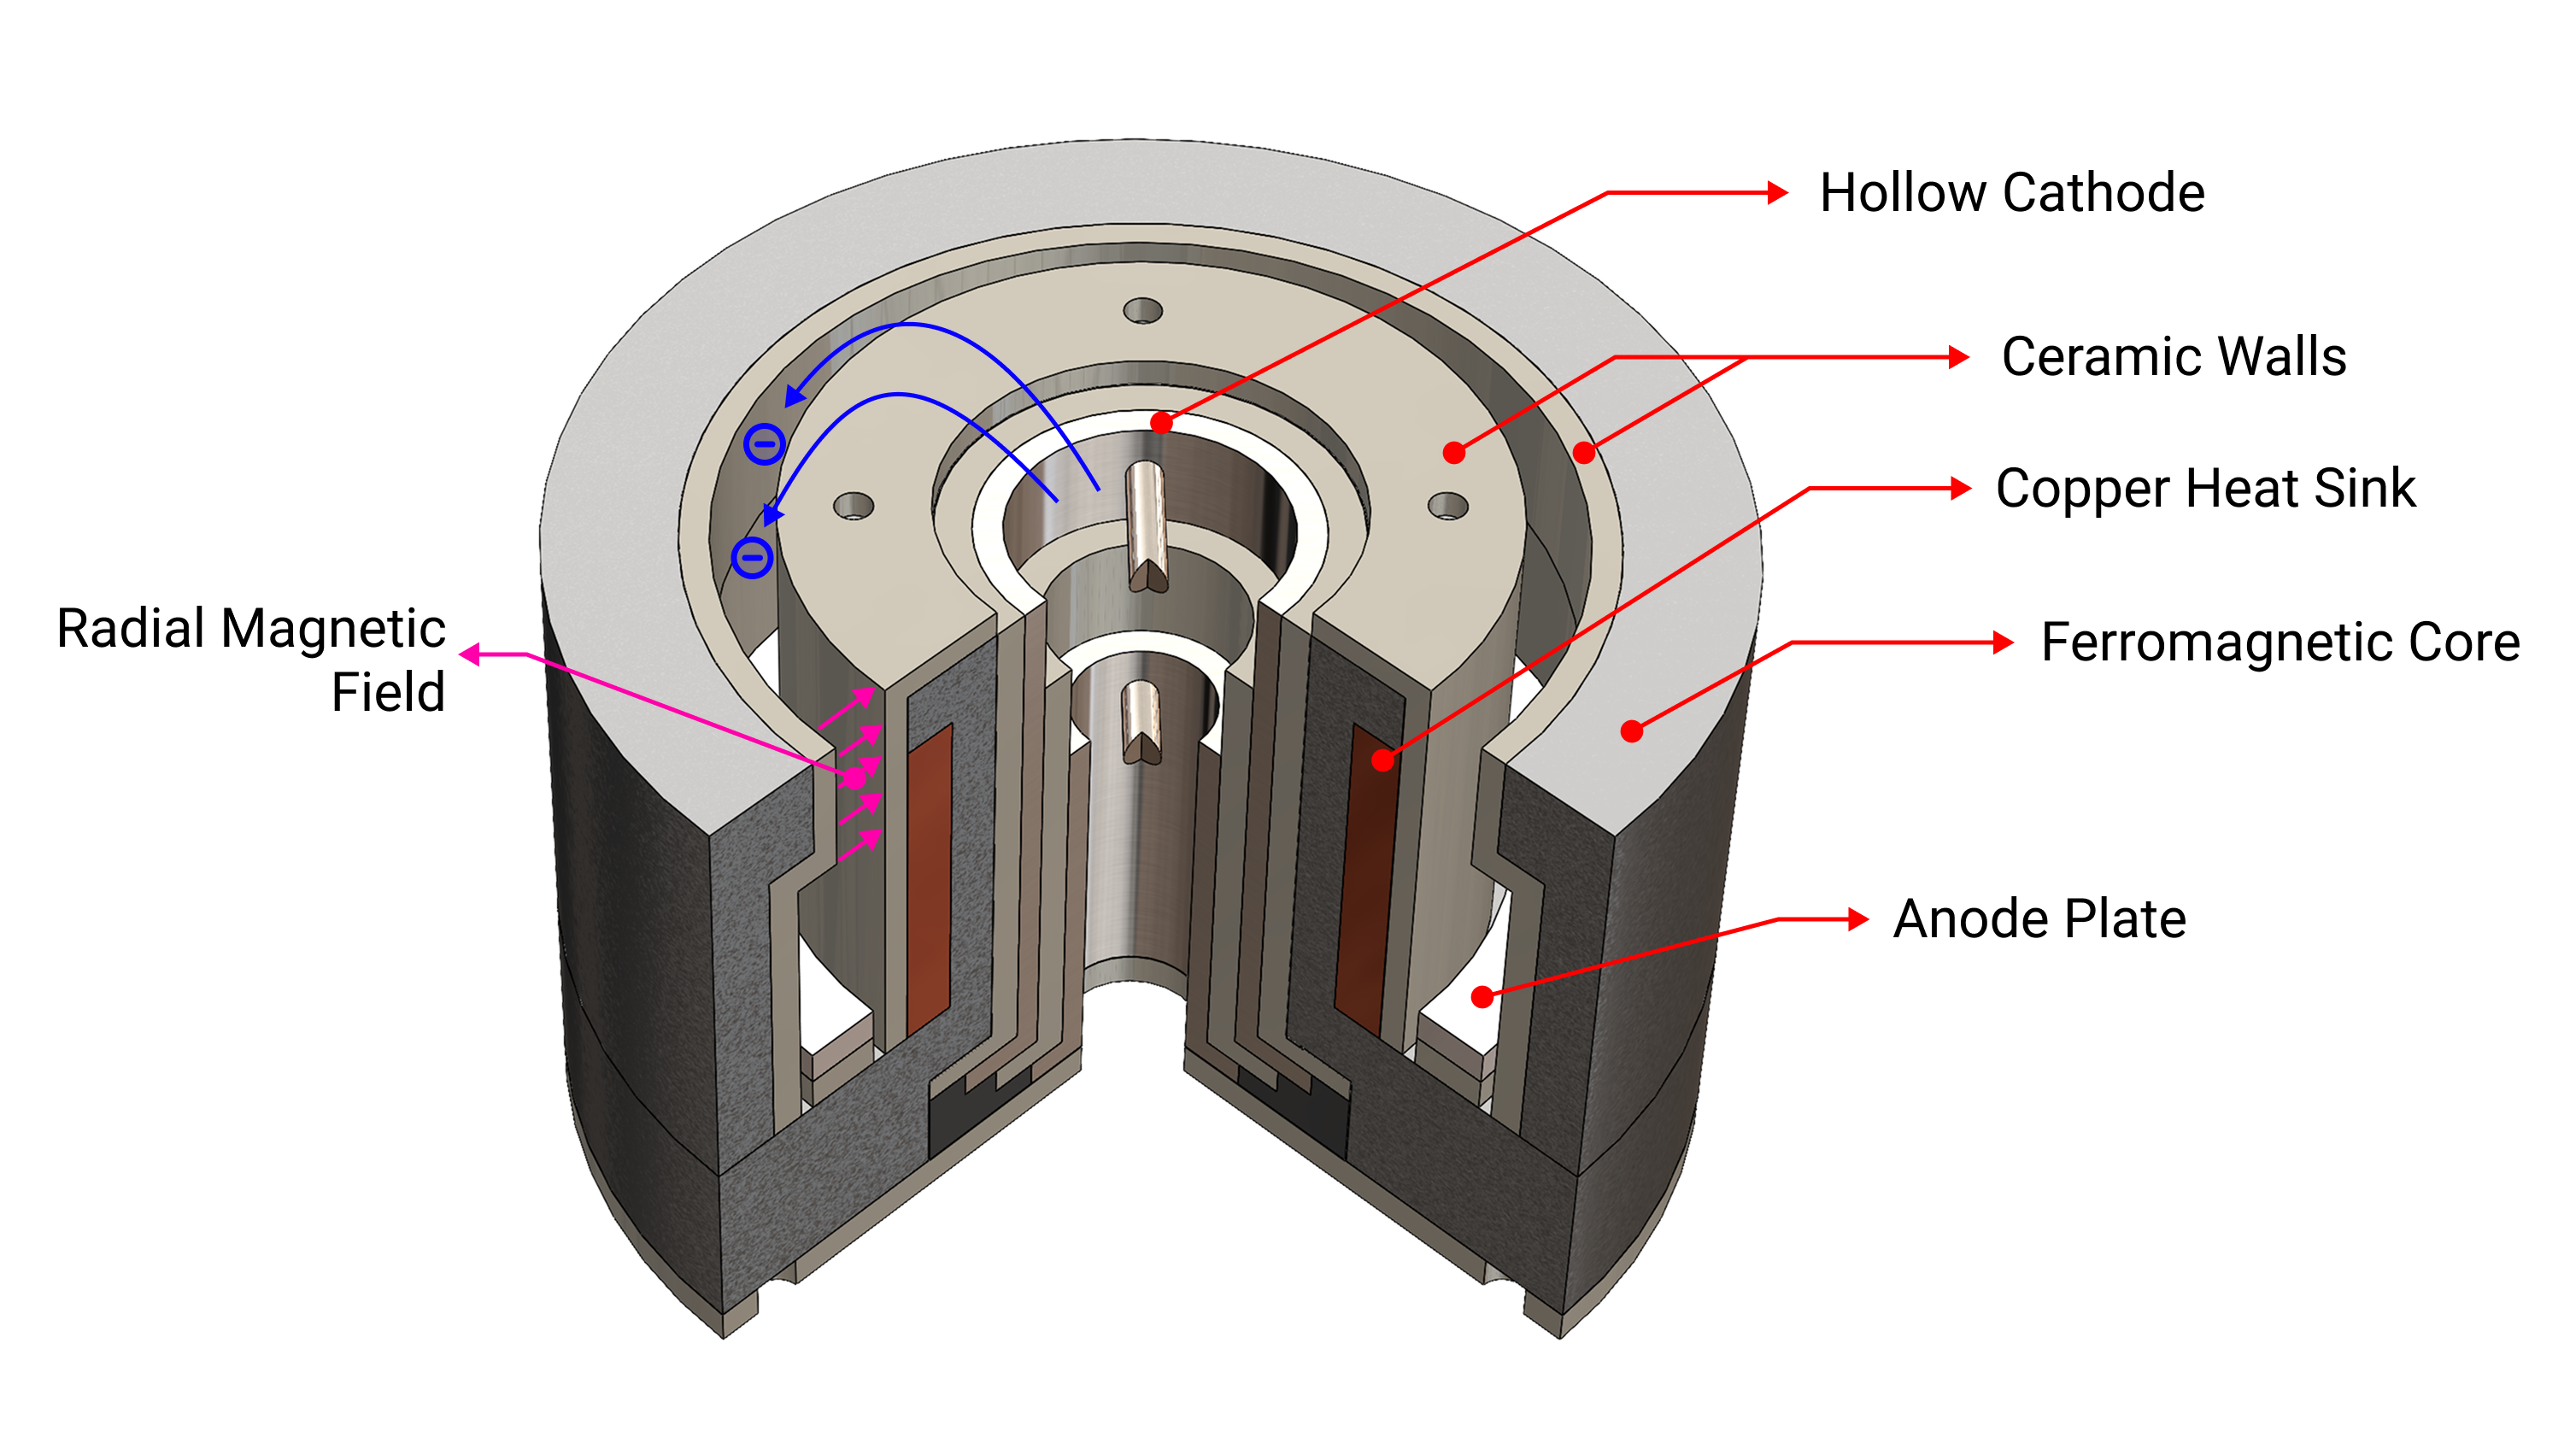
\includegraphics[width=1.0\textwidth]{images/Concepts/final concept.png}
    \captionsetup{justification=centering}
    \caption{Final Concept Diagram}
    \label{fig:final_concept}
\end{figure}

% DESIGN DEVELOPMENT
\section{Design Development}

% PROTOTYPES AND DESIGN VERIFICATION
\section{Prototypes and Design Verification}

% TESTING
\section{Testing}

% CLOSING REMARKS
\section{Closing Remarks}


% PROJECT MANAGEMNET
\section{Project Management}

% ---------------------APPENDIX---------------------
\appendix
\newpage
\section{List of Figures}
Here you can include additional figures, tables, or explanations.

\newpage
\section{List of Tables}
Detailed derivations go here.

\newpage
\section{Code Snippets}

\begin{verbatim}
for i in range(10):
    print(i)
\end{verbatim}

% ---------------------CITATIONS---------------------

\newpage
\printbibliography

\end{document}  
